% Metódy inž7inierskej práce

\documentclass[10pt,twoside,slovak,a4paper]{article}

\usepackage[slovak]{babel}
%\usepackage[T1]{fontenc}
\usepackage[IL2]{fontenc} % lepšia sadzba písmena Ľ než v T1
\usepackage[utf8]{inputenc}
\usepackage{graphicx}
\usepackage{url} % príkaz \url na formátovanie URL
\usepackage{hyperref} % odkazy v texte budú aktívne (pri niektorých triedach dokumentov spôsobuje posun textu)

\usepackage{cite}
%\usepackage{times}

\pagestyle{headings}

\title{Možnosti a efektívnosť získania jazykových znalostí prostredníctvom
e-learningu\thanks{Semestrálny projekt v predmete Metódy inžinierskej práce, ak. rok 2020/21, vedenie: Ing. Fedor Lehocki }} % meno a priezvisko vyučujúceho na cvičeniach

\author{Richard Szarka\\[2pt]
	{\small Slovenská technická univerzita v Bratislave}\\
	{\small Fakulta informatiky a informačných technológií}\\
	{\small \texttt{xszarkar@stuba.sk}}
	}

\date{\small 7. október 2020} % upravte



\begin{document}

\maketitle

\begin{abstract}
Získavanie vedomostí cez internet je čoraz bežnejšie. Jednou z najžiadanejších oblastí v e-learningu je najmä získavanie jazykových znalostí. Na osvojenie si jazyka v kontaktnom vzdelávaní je potrebné precvičovať jazyk rôznymi metódami rovnako ako pri autonómnom vzdelávaní pomocou e-learningu. Cieľom tejto práce je definovať a porovnať metódy nadobúdania jazykových zručností prostredníctvom e-learningu. V práci si rozoberieme metódy, ako napríklad úlohy zadávané softwarom (Duolingo), aktívnu komunikáciu s osobou, ktorá daný jazyk už ovláda (Tandem, HelloTalk) alebo pasívnu komunikáciu so skupinou ľudí s rovnakým cieľom (jazykové blogy). Zameriame sa na to, aké výhody majú jednotlivé metódy, ktoré konkrétne jazykové zručnosti rozširujú, ale aj aká je efektívnosť nadobúdania jazykových znalostí cez e-learning.
\end{abstract}

\section{Úvod} %1

\section{Čo je e-learning?}%2
Učenie sa v dnešnej dobe je tak jednoduché, že stačí na to použitie hocijakého komunikačného zariadenia, ktoré vám je schopné dávať informácie\cite{vyhody}. Pojem e-learning je bežne vysvetlený ako vedomé použitie kominikačných a sieťových technológií v učení a učení sa. Alternatívnou definiciou e-learningu môže byť: aplikovanie elektronických systémov, ako internet a pocitace, ktoré šetria čas a financie \cite{efektivnost}. 

\subsection{Výhody e-learningu}%2.1
Ku každej novej technológii patria výhody. E-learning priniesol mnohé výhody v učení a výučby, ktoré zahrňujú aj výučbu jazykov. Medzi mnohé z výhod patrí :
\begin{itemize}
\item E-learning je rýchly a dynamický a znižuje výdavky (ako napríklad cestovanie) \cite{efektivnost}
\item Lekcie sú pripravované rôznými učiteľmi \cite{efektivnost}
\item Interaktívne cvičenia zvyšujú motiváciu študentov \cite{vyhody}
\item Aktivity e-learningu prinášajú rôzne skúsenosti rôznym ľuďom a takéto aktivity pomáhajú lahšiemu učeniu \cite{vyhody}
\item Je to druh kooperatívneho vzdelávania \cite{efektivnost}
\end{itemize}

\subsection{Nevýhody e-learningu}%2.2
Každá technológia, ktorá prináša výhody, prináša so sebou aj nejaké nevýhody. Jedny z mnohých nevýhod e-learningu a aj nevýhod výučby jazykov sú :

\begin{itemize}
\item Jazykové a kultúrne rozdiely \cite{efektivnost}
\item Technologické problémy u študentov sú často technofóbia a nedostupnosť požadovaných technológií \cite{nevyhody}
\item Znížená socialna a kultúrna interakcia ako je napríklad reč tela \cite{nevyhody}
\item Technické limitácie\cite{efektivnost}
\end{itemize}

\section{Najznámejšie a najobľúbenejšie e-learningové možnosti učenia sa jazyka}%3
Najväčší rozmach získavania jazykových vedomostí zažívajú v dnešnej dobe hlavne rôzne mobilné aplikácie. Mnohé z nich sú považované aj za edukatívne hry, ako napríklad DuoLingo. Atraktivita týchto aplikácii je spôsobená ľahkou dostupnosťou a tým, že ich používanie aplikácií je zadarmo (občasné reklamy). Avšak, v ústraní neostali ani platené kurzy a jazykové blogy.

\subsection{Aplikácia DuoLingo}%3.1
DuoLingo je mobilná aplikácia na vzdelávanie masy ľudí. Umožňuje získavanie jazykových znalostí pomocou rôznych kurzov. Užívateľ si vyberie jazyk ktorým hovorí (ak je dostupný) a jazyk v ktorom by sa chcel zdokonaliť. Momentálne je 45 kurzov do rôznych iných jazykov ak si vyberiete možnosť že hovoríte po anglicky. Výber jazyka ktorým užívateľ už hovorí je obmedzenejší (21) a nie je rovnaký počet kurzov v každom jazyku.Ak výber jazyka ktorému rozumiete je nemčina tak máte na výber 4 kurzy(https://www.duolingo.com/courses).
DuoLingo periodicky pridáva nové kurzy a aktívne zveľaduje rozsah užívateľov, ktorým táto aplikácia môže byť užitočná\ref{duo-uzivatelia}.\\ Tento vývoj DuoLinga je vidieť aj na množstve aktívnych používateľov aplikácie. Pomerne nové vybavenie na rozvoj jazyka užívateľa je"Duolingo stories" (https://www.duolingo.com/stories/). Užívateľa zaujmú príbehy kde musí on zadávať gramaticky správne odpovede alebo vybrať odpoveď, ktorá sa hodí do daného kontextu. Výhoda je aj udržanie pozornosti pomocou nepredvýdaných a zaujímavých koncov príbehov.


\begin{figure} %obrázok
\centering
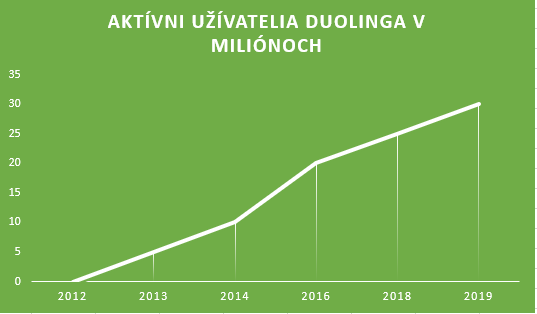
\includegraphics[width=\textwidth]{duolingo.png}
\caption{popis obrázka}
\label{duo-uzivatelia}
\end{figure}

Používanie aplikácie Duolingo je jednoduché a zameriava sa, na takmer všetky vekové kategórie\cite{duolingo}.
\subsection{Aplikácia Hellotalk}

\subsection{Aplikácia Tandem}

\subsection{Jazykové blogy}

\subsection{Online kurzy}

\section{Efektívnosť e-learningu}

\section{Záver}

\bibliography{zdroje_literatura}
\bibliographystyle{plain}
\end{document}
